


%\begin{enumerate}
%	\item $N$:  stati nascosti
%	\item $M = |V|$: alfabeto osservazione
%%	\item $\mathbf{A} = \{a_{ij}\}$: probabilit� di transizione \\
%%	\item $N = 4$ , stati $S = \{HS, FF, HO, FO\}$
%%	\item $M = |V|$, valori di osservazione segnale giroscopico 
%	
%
%%	$\omega (^\circ/s)$ $a_{ij} = \wp[q_t = S_j | q_{t-1} = S_i]$
%%		\begin{equation}
%			%\begin{split}
%%			$A = \,& \{a_{ij}\}\; 	
%\item $\mathbf{B} = \{b_j(k)\}$: probabilit� di emissione\\ 
%%			\end{split}
%%		\end{equation}$b_j(k) = \wp[v_k \; \text{all'istante } t | q_t = s_j] $
%%	delle osservazioni $\omega$ di ciascuno stato $S_i$
%%	\begin{equation}
%%\begin{split}
%%$\mathbf{B} = \{b_j(k)\}\;	
%\item $\pi = \{\pi_i\}$: probabilit� a priori \\
%%\end{split}	 
%%\label{eq:emissionMtxDef}
%%\end{equation}	
%%		\begin{equation}
%%	B = b_j(x) = \mathcal{N}(x,\mu_j,\sigma_j) = \frac{1}{\sigma_j\sqrt{2\pi}}\textbf{e} ^{-\frac{(x-\mu_j)^2}{2 \sigma_j^2}}\quad
%%		\text{per} 1 \leq j \leq N \nonumber
%%		\end{equation}$\pi_i = \wp(q_1 = S_i)$\\\vspace{.5cm}
%%	\begin{equation}
%%\begin{split}
%$	\mathbf{\pi} = \{p_i\}\; $1\leq i,j \leq N $ e $1\leq k \leq M$ 
%%\end{split}	
%%\label{eq:prior}
%%\end{equation}
%\end{enumerate}	


\frame{
%\subsection{}
\frametitle{Parte I. HMM per l'analisi della deambulazione: definizione}

\begin{columns}
\column{.6\textwidth}

	\begin{figure}
	\centering
	  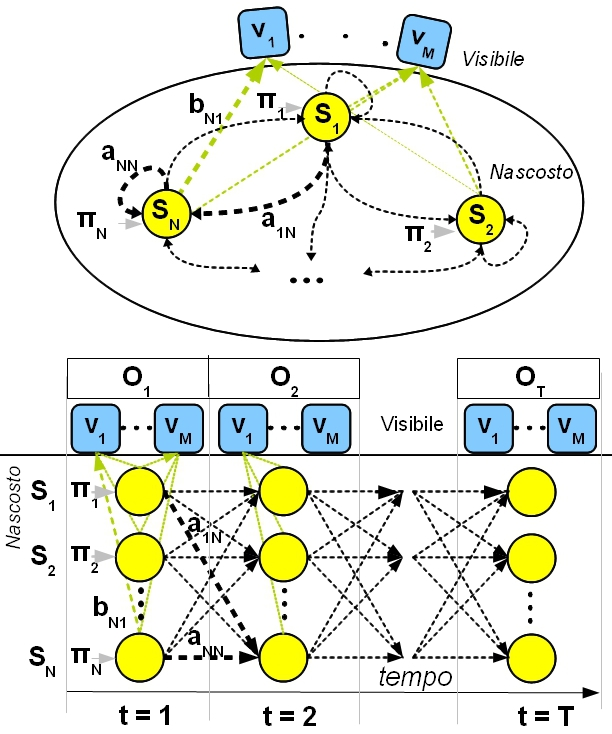
\includegraphics[width=.9\textwidth]{imgs/descreteMarkovProcesses2.jpg}	
	\end{figure}

\column{.5\textwidth}

	\tiny{
	HMM $= <N, M, \mathbf{A}, \mathbf{B}, \mathbf{\pi}>$
dove: 

\begin{enumerate}
	\item $N = |S|$: stati nascosti
	\item $M = |V|$:  alfabeto osservazione
	\item $\mathbf{A}\{a_{ij}\}$: probabilit� di transizione 
				$a_{ij} = \wp[q_t = S_j | q_{t-1} = S_i]$
	\item $\mathbf{B}$ :probabilit� di emissione
				$b_j(k) = \wp[v_k \; \text{all'istante } t | q_t = s_j] $
	\item $\mathbf{\pi}$: probabilit� a priori
				$\pi_i = \wp(q_1 = S_i)$
				
\end{enumerate}

\end{columns}
}

}

